
\chapter{Discovering (Setting Limit for) \boldmath{\Bmumumu} at LHCb}

\label{chap:sel}

\textit{LHCb's flagship analyses contain several muons in the final state coming from differently flavoured $B$ mesons. Despite being in this category, search for \Bmumumu is limited by the rareness of its occurence as well as different backgrounds that can mimique its signature in the detector. Moreover, presence of invisible neutrino does induce uncertainties into reconstruction. This \autoref{chap:sel} will concentrate on characterisation of backgrounds as well as selection that is performed in order to reduce the backgrounds.}


\section{Topology of \Bmumumu at LHCb}

At \Gls{LHCb}, \Bpm particle will travel less than a milimetre in the laboratory frame of reference before it decays into its decay products. This allows reconstruction of a primary vertex \Gls{PV} and its decay vertex, \textit{secondary vertex} \Gls{SV}. By joining these vertices, direction as well as lenght of the \Bpm flight can be established. The schematic diagram can be seen in \autoref{fig:sigtopo}.

\begin{figure}
  \centering
  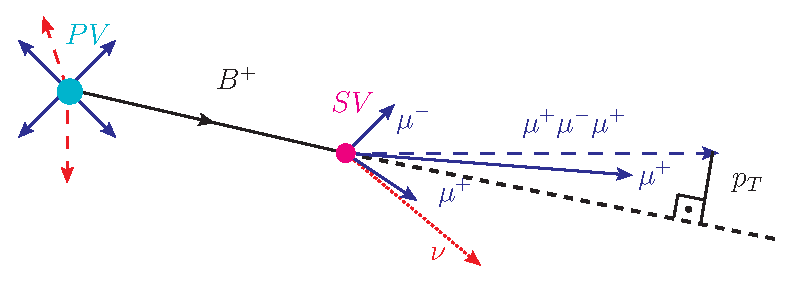
\includegraphics[scale = 1.0]{figs/sel/DecReco_fin.eps}
	\caption{Schematic view of \Bmumumu at \Gls{LHCb}.}
  \label{fig:sigtopo}
\end{figure}

